\documentclass[12pt]{article}

\usepackage{answers}
\usepackage{setspace}
\usepackage{graphicx}
\usepackage{enumitem}
\usepackage{multicol}
\usepackage{mathrsfs}
\usepackage[margin=1in]{geometry} 
\usepackage{amsmath,amsthm,amssymb}
\usepackage[ngerman]{babel}

\newcommand{\N}{\mathbb{N}}
\newcommand{\Z}{\mathbb{Z}}
\newcommand{\C}{\mathbb{C}}
\newcommand{\R}{\mathbb{R}}

\DeclareMathOperator{\sech}{sech}
\DeclareMathOperator{\csch}{csch}

\newenvironment{theorem}[2][Theorem]{\begin{trivlist}
		\item[\hskip \labelsep {\bfseries #1}\hskip \labelsep {\bfseries #2.}]}{\end{trivlist}}
\newenvironment{definition}[2][Definition]{\begin{trivlist}
		\item[\hskip \labelsep {\bfseries #1}\hskip \labelsep {\bfseries #2.}]}{\end{trivlist}}
\newenvironment{proposition}[2][Proposition]{\begin{trivlist}
		\item[\hskip \labelsep {\bfseries #1}\hskip \labelsep {\bfseries #2.}]}{\end{trivlist}}
\newenvironment{lemma}[2][Lemma]{\begin{trivlist}
		\item[\hskip \labelsep {\bfseries #1}\hskip \labelsep {\bfseries #2.}]}{\end{trivlist}}
\newenvironment{exercise}[2][Exercise]{\begin{trivlist}
		\item[\hskip \labelsep {\bfseries #1}\hskip \labelsep {\bfseries #2.}]}{\end{trivlist}}
\newenvironment{solution}[2][Solution]{\begin{trivlist}
		\item[\hskip \labelsep {\bfseries #1}]}{\end{trivlist}}
\newenvironment{problem}[2][Problem]{\begin{trivlist}
		\item[\hskip \labelsep {\bfseries #1}\hskip \labelsep {\bfseries #2.}]}{\end{trivlist}}
\newenvironment{question}[2][Question]{\begin{trivlist}
		\item[\hskip \labelsep {\bfseries #1}\hskip \labelsep {\bfseries #2.}]}{\end{trivlist}}
\newenvironment{corollary}[2][Corollary]{\begin{trivlist}
		\item[\hskip \labelsep {\bfseries #1}\hskip \labelsep {\bfseries #2.}]}{\end{trivlist}}

\begin{document}
	\title{Künstliche Intelligenz 2 - Zusammenfassung}
	\author{Michael Gabler}
	\maketitle
	\tableofcontents
	\newpage
	
	\section{Unsicheres Wissen und Schließen}
	Logik benötigt exakte Regeln, die immer wahr sind. Oft nicht gegeben (zu wenig Daten, keine Regeln möglich) $\rightarrow$ wahrscheinlichkeitsbasiertes Entscheiden. Ein Agent benötigt dazu Präferenzen, wie nützlich verschiedene Ziele sind und die Wahrscheinlichkeiten, diese Ziele zu erreichen.\\
	\textbf{Rationalität} = wähle Aktion mit der größten erwarteten Nützlichkeit
	
	\subsection{Wahrscheinlichkeitsrechnung}
	\textbf{unbedingte Wahrscheinlichkeit} $P(A)$\\
	\textbf{Wahrscheinlichkeitsverteilung} $P(Wetter) = (0,7; 0,2; 0,008; 0,02)$\\
	\textbf{Operanden} $\wedge$ = und, $\vee$ = oder\\
	\textbf{Bedingte Wahrscheinlichkeit} wie wahrscheinlich ist $A$ wenn $B$ wahr ist:
	$$P(A|B) = \frac{P(A \wedge B)}{P(B)} \Leftrightarrow P(A \wedge B) = P(A|B) P(B)$$\\
	$P(A \vee B) = P(A) + P(B) - P(A \wedge B)$\\
	\textbf{Apriori-Wahrscheinlichkeit} Wahrscheinlichkeit für ein Ereignis unabhängig von den anderen: $P(X) = \sum_y P(X,y)$ (Marginalization) oder $P(X) = \sum_y P(X|y) P(y)$ (Conditioning)\\
	\textbf{Unabhängige Variablen} Für Variablen, deren Ereignisse unabhängig voneinander eintreten gilt: $P(a|b) = P(a)$\\
	\textbf{Bayes' Theorem} $P(B|A) = \frac{P(A|B) P(B)}{P(A)}$ wird verwendet zur Herleitung nicht bekannter, abhängiger Wahrscheinlichkeiten\\
	\textbf{Naives Theorem von Bayes} Annahme: Symptome $S_i$ untereinander unabhängig (oft nicht gegeben), Vollständigkeit der Diagnosen $D_i$
	$$P(D_i|S_1 \wedge ... \wedge S_m) = \frac{P(D_i) P(S_1|D_i) ... P(S_m|D_i)}{\sum_{j=1}^{n} P(D_j) P(S_1|D_j) ... P(S_m|D_j)} = \alpha P(D_i) P(S_1|D_i) ... P(S_m|D_i)$$
	Dabei ist $\alpha$ eine Normierungskonstante, so dass die Summer aller Wahrscheinlichkeiten 1 ergibt.\\
	\textbf{Numerische Variablen} Annahme: alle Variablen haben diskrete Werte. Kontinuierliche Variablen werden diskretisiert oder Verwendung, wenn Verteilungsfunktion bekannt ist.
	
	\subsection{Probabilistische/Bayessche Netze}
	Theorem von Bayes behandelt alle Symptome als voneinander unabhängig. Probabilistische Netze (gerichtete, azyklische Graphen) stellen Abhängigkeiten dar.\\
	\textit{einfach verbunden}: es gibt nur einen Pfad zu einem Knoten, \textit{mehrfach verbunden}: ex existieren mehrere Pfade zum gleichen Knoten\\
	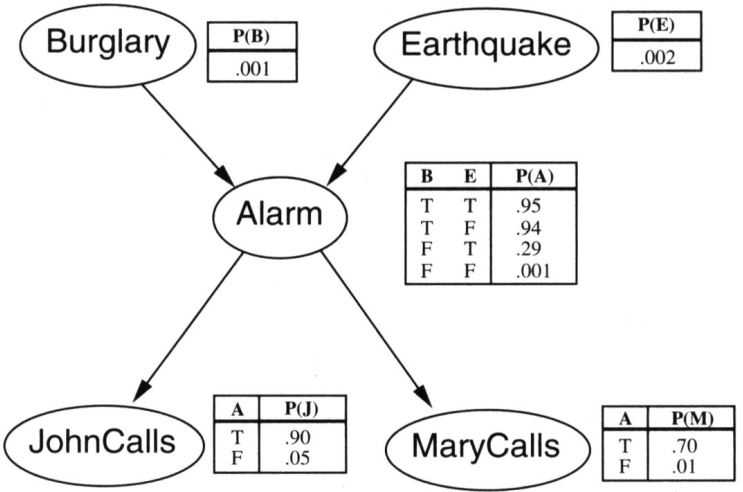
\includegraphics[width=\textwidth]{figures/probabilistisches-netz.JPG}\\
	\textbf{Konstruktion von probabilistischen Netzen}
	\begin{enumerate}
		\item Wähle geeignete Zufallsvariable
		\item Wähle Reihenfolge der Variablen (Wichtig für Größe des Netzes)
		\item Solange Variablen noch nicht im Netz sind:
			\subitem Nimm nächste Variable $X_i$
			\subitem Setze die Eltern von $X_i$ auf eine minimale Menge von bereite im Netz vorhandenen Knoten
			\subitem Definiere die Wahrscheinlichkeitstabelle für $X_i$
	\end{enumerate}
	Es ermöglicht die Wahrscheinlichkeitsberechnung jeder vollständigen Knotenbelegung.\\
	Beispiel: $$P(J \wedge M \wedge A \wedge \bar{B} \wedge \bar{E}) = P(J|A) P(M|A) P(A|\bar{B} \wedge \bar{E}) P(\bar{B}) P(\bar{E}) = 0,9 \cdot 0,7 \cdot 0,0001 \cdot 0,999 \cdot 0,998 = 0,000628$$
	\textbf{Unabhängigkeit} $X$ ist unabhängig von seinen Nichtnachfolgern $Z_{ij}$, wenn seine Eltern $U_i$ bekannt sind (siehe rechts).\\
	$X$ ist unabhängig von allen anderen Knoten, wenn seine Eltern $U_i$, seine Kinder $Y_i$ und deren andere Eltern $Z_{ij}$ bekannt sind $\Rightarrow$ Markov blanket (siehe links)\\
	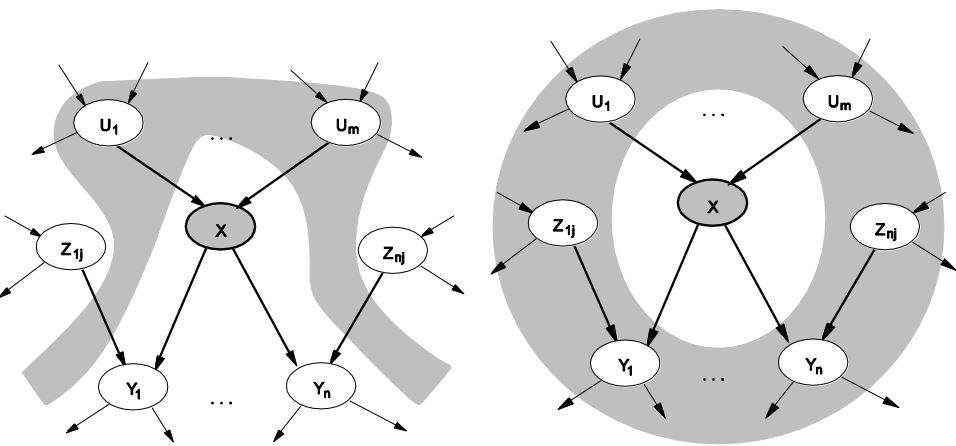
\includegraphics[width=\textwidth]{figures/markov-blanket.JPG}
	\textbf{Enumerate-Joint-Ask} Berechnung von nicht vollständigen Knotenbelegungen $\rightarrow$ bilde Summe über unbekannte Möglichkeiten: $$P(B|J \wedge M) = \alpha P(B,J,M) = \alpha \sum_e \sum_a P(B \wedge e \wedge a \wedge J \wedge M)$$
	$\Rightarrow$ Komplexität für $n$ boolsche Variablen: $O(n2^n)$\\
	\textbf{Verbesserungen} Speichern von Berechnungen, Verschiebung von Termen vor die Summe, Irrelevante Variablen die 1 ergeben erkennen und eliminieren, Zusammenfassung von Knoten in mehrfach verbundenen Netzen\\
	\textbf{Stochastische Simulation} Führe mehrere Simulationsläufe mit Zufallswerten durch und berechne aus den Häufigkeiten die Wahrscheinlichkeiten.
	\begin{itemize}
		\item Direct Sampling: wähle Werte in topologischer Reihenfolge der Wahrscheinlichkeitstabelle entsprechend $\rightarrow$ erfordert viele Läufe für seltene Ereignisse
		\item Rejection Sampling: wie Direct Sampling, aber nicht relevante Läufe werden ignoriert
		\item Likelihood Weighting: setze interessante Werte und gewichte entsprechend der Wahrscheinlichkeitstabellen $\rightarrow$ effizient, kann aber nicht alles gleichzeitig berechnen
		\item Markov Chain Monte Carlo (MCMC): wähle Wertebelegung entsprechend der Vorgaben, restliche Knoten werden zufällig entsprechend ihrer Markov Blanket gewählt
	\end{itemize}
	\textbf{Berechnung der wahrscheinlichsten Sequenz} Wahrscheinlichkeiten für Zustände in Abhängigkeit einer Variable gegeben, Wahrscheinlichkeit für Auftreten des Folgezustandes gegeben. Berechne wahrscheinlichste Sequenz durch durchrechnen.\\
	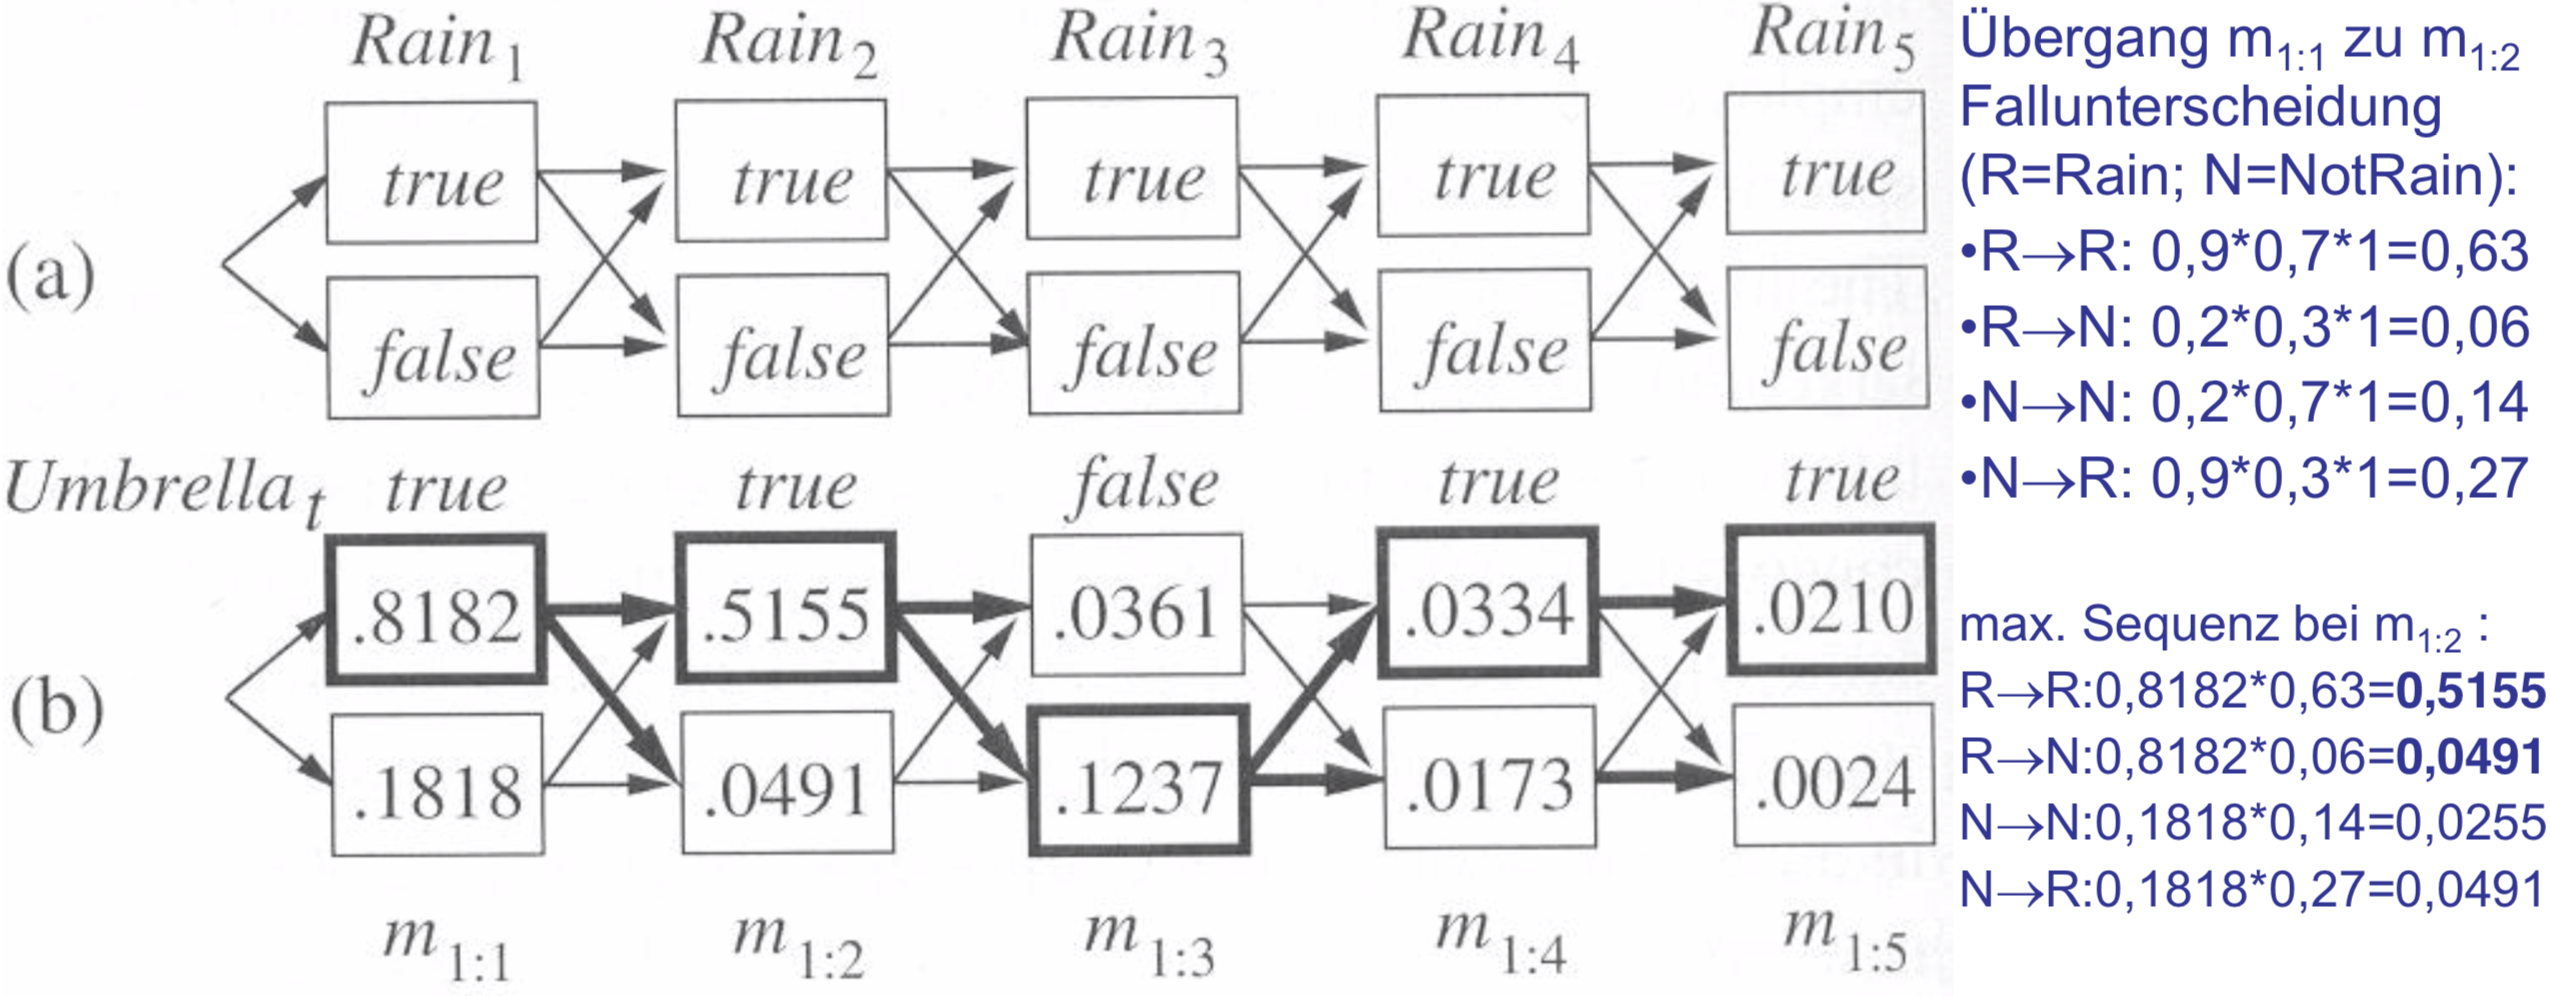
\includegraphics[width=\textwidth]{figures/wahrscheinlichste-sequenz.png}\\
	\textbf{Hidden Markov Model} Reduktion aller Variable auf eine einzige, die alle Zustände abbildet $\rightarrow$ wird zur Abbildung von Phonemen (Lauten) auf Wörter verwendet\\
	\textbf{Kalman Filter} Schätzung des Zustandes eines physischen Systems anhand verrauschter Beobachtungen (z.B. Flugzeuge auf Radarschirm)\\
	\textbf{Viterbi Algorithmus} rekursives Vorgehen
	
	\subsection{Entscheiden}
	\textbf{Erwartete Nützlichkeit} Ziel einer Entscheidung sollte die Maximierung der erwarteten Nützlichkeit $EU$ sein. Diese berechnet sich unter der Vorbedingung $E$ für eine Aktion $A$ mit $i$ verschiedenen Ergebnissen wie folgt: $EU(A|E) = \sum_i P(Ergebnis_i(A)|E, Tue(A)) U(Ergebnis_i(A))$ mit $U$ als Nützlichkeit\\
	\textbf{Axiome der Nützlichkeitstheorie}
	\begin{itemize}
		\item Reihenfolge: $(A \succ B) \vee (B \succ A) \vee (A \sim B)$
		\item Transitivität: $(A \succ B) \wedge (B \succ C) \Rightarrow (A \succ C)$
		\item Kontinuität: $A \succ B \succ C$ Agent ist unsicher, wenn er $B$ sicher bekommt, $A$ aber nur mit Wahrscheinlichkeit $p$ und $C$ mit $1-p$
		\item Ersetzbarkeit: gleiche Entscheidung für komplexere Lotterien, die $A$ und $B$ enthalten wie zwischen nur $A$ und $B$
		\item Monotonie: zwei Lotterien mit der Nützlichkeit $A$ und $B$. Wenn $A$ besser als $B$, dann muss auch andere Lotterie bevorzugt werden, die $A$ mit höherer Wahrscheinlichkeit nutzt
		\item Zerlegbarkeit: Komplexe Lotterien können vereinfacht werden, da der Agent keine Lotterie bevorzugen sollte, nur weil er mehr Wahlmöglichkeiten hat
	\end{itemize}
	\textbf{Probleme} Beste Wahrscheinlichkeiten oft überschätzt; Mensch entscheidet nicht rational\\
	strikt dominant: in jedem Attribut besser; stochastisch dominant: besser für jedes Wahrscheinlichkeitsniveau\\
	\textbf{Entscheidungsnetze} Erweiterung von probabilistischen Netzen um Entscheidungs- und Nützlichkeitsknoten. $\rightarrow$ Entscheidungsknoten beeinflussen die Zufallsvariablen und damit die Nützlichkeit. Vorgehen zur Auswertung:
	\begin{enumerate}
		\item Setze Zufallsvariablen entsprechend dem aktuellen Zustand
		\item Für jede mögliche Aktion des Entscheidungsknotens:
			\subitem Setze den Entscheidungsknoten auf diesen Wert
			\subitem Berechne Wahrscheinlichkeiten der Eltern-Knoten des Nützlichkeitsknoten mit einem Inferenz-Algorithmus für probabilistische Werte
			\subitem Berechne Nützlichkeit der Aktion
		\item Wähle Aktion mit größter Nützlichkeit
	\end{enumerate}
	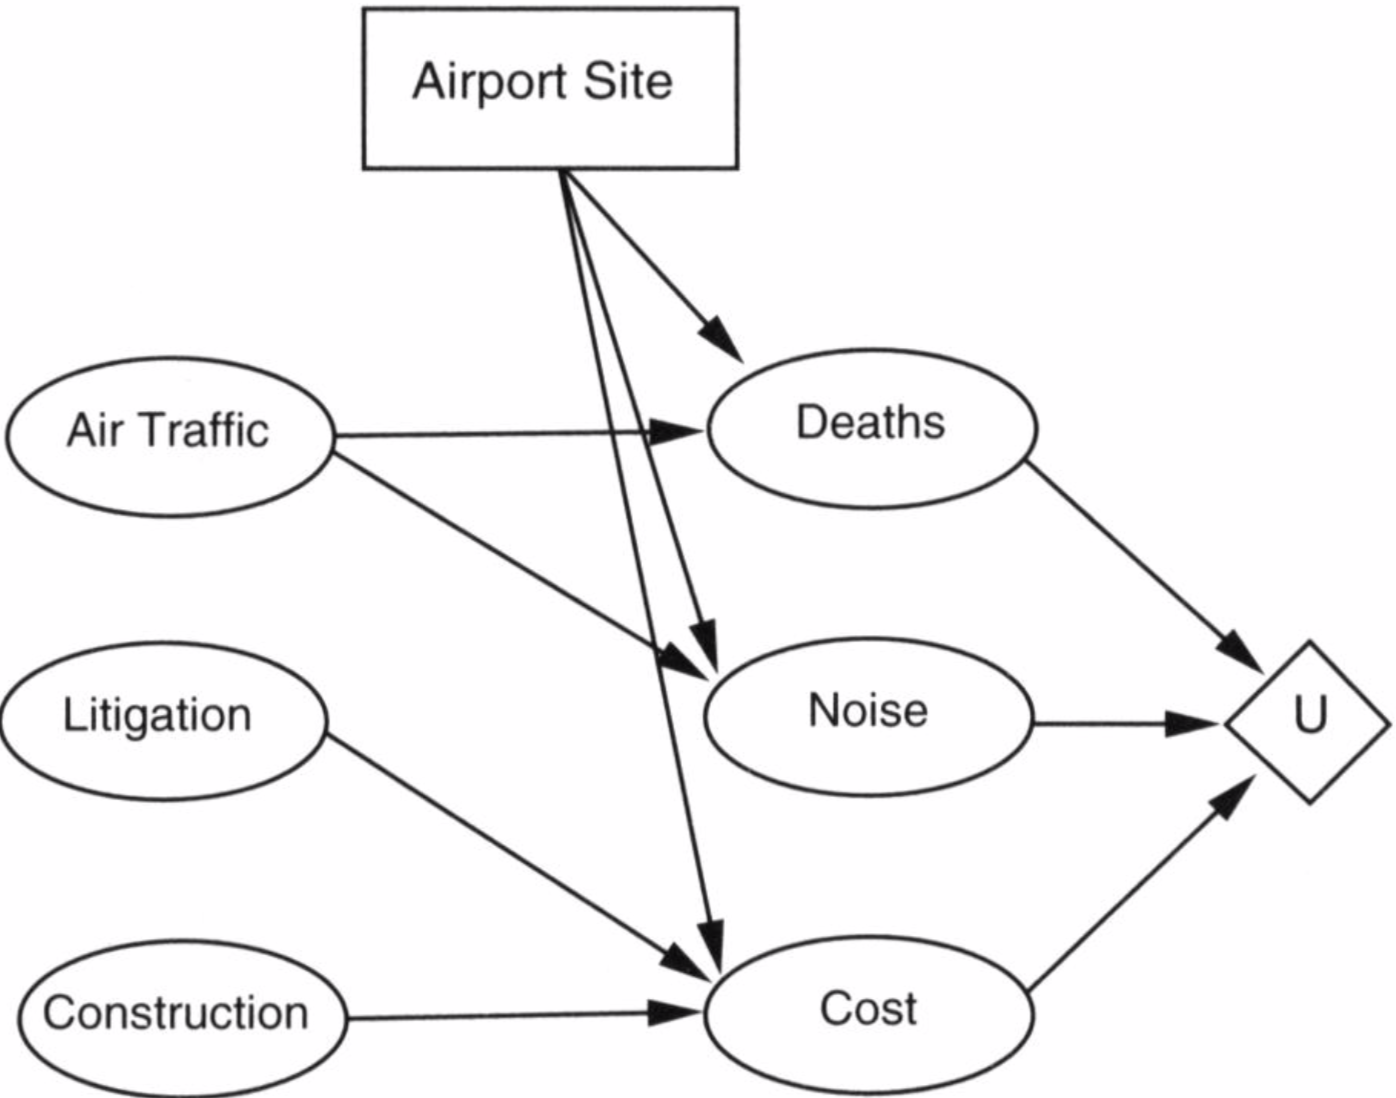
\includegraphics[width=0.5\textwidth]{figures/entscheidungsnetz.png}\\
	Bewertung der Nützlichkeit ist genauer mit mehr Informationen. Nützlichkeit der Information ist immer positiv, nicht additiv und kann berechnet werden.
	
	\section{Lernen}
	Lernende Agenten haben \textbf{Verhaltenskomponente} (Problemlöser), \textbf{Lernkomponente} (Verbesserung der Verhaltenskomponente), \textbf{Kritikkomponente} (Bewertung des Verhaltens) und einen \textbf{Problemgenerator} (Exploration). Lernen kann dabei als Lernen der Repräsentation einer Funktion betrachtet werden.\\
	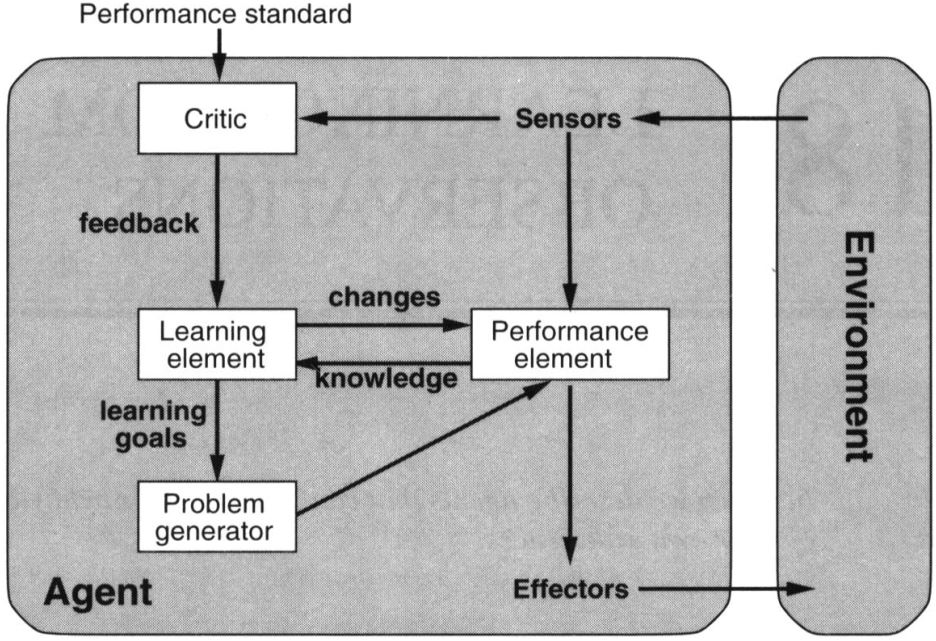
\includegraphics[width=\linewidth]{figures/lernender-agent.JPG}\\
	\textbf{Lernarten}
	\begin{enumerate}
		\item Geführtes Lernen (Supervised learning)
		\item Verstärkungslernen (reinforcement learning)
		\item Ungeführtes Lernen (unsupervised learning)
		\item Teilgeführtes Lernen (semi-supervised learning)
	\end{enumerate}
	\textbf{Lernen einer Funktion} Gegeben Ausgaben einer Funktion, die approximiert werden soll. Aufteilung in Trainingsmenge und Testmenge. Bei \textbf{endlicher} Ausgabemenge $\Rightarrow$ \textbf{Klassifikation}, bei \textbf{kontinuierlicher} Ausgabe $\Rightarrow$ \textbf{Regession}\\
	\textbf{Auswahl verfügbarer Hypothesen} (gelernte Funktionen): bevorzuge einfache Hypothese (Ockham's razor) $\Rightarrow$ Präferenzannahme (\textbf{Bias})\\
	\textbf{Entropie}: Informationsmaß für die Unsicherheit einer Zufallsvariable. Wie viel Bit werden benötigt, um die Zustände zu repräsentieren? (z.B. Münze werfen $\rightarrow$ 1 Bit, 4-seitiger Würfel $\rightarrow$ 2 Bit, aber Münze mit 99 \% Wahrscheinlichkeit für Zahl $\rightarrow > 0$). Allgemein: Entropie $H$ der Zufallsvariablen $V$, deren Werte $v_k$ sind
	$$H(V) = \sum_k P(v_k) \log_2 \frac{1}{P(v_k)} = - \sum_k P(v_k) \log_2 P(v_k)$$
	Damit ergibt sich eine Entropie $B$ für boolsche Variablen, die mit der Wahrscheinlichkeit $q$ wahr sind: $B(q) = - (q \log_2 q + (1-q) \log_2 (1-q))$.\\
	\textbf{Overfitting} beschreibt das zu starke Anpassen eines Lernmodells an die Testdaten, wodurch die Klassifikation auf realen Daten schlecht funktioniert.\\
	\textbf{Pruning} Entfernen irrelevanter Attribute (zufällige Aufteilung) $\rightarrow$ Chi-Quadrat-Test\\
	\textbf{Cross-Validation} Überprüfe Bewertungsgenauigkeit mit unabhängigem Testset an Daten (reservierter Teil der Trainingsdaten) $\rightarrow$ k-fold Cross Validation reserviert für jeden der $k$ Trainigsdurchgänge $\frac{1}{k}$ der Trainingsdaten als Testdaten\\
	\textbf{Loss Function} (Verlustfunktion) ist ein Maß dafür, wie viele Fehler das aktuellen Modell bei der Klassifizierung macht (kann z.B. nach Schwere des Fehlers gewichtet werden)
	
	\subsection{Lernen von Entscheidungsbäumen}
	Für den Mensch einfach verständlich, Ausgabe ist Ja/Nein-Entscheidung (boolean). Für $n$ verschiedene boolsche Eingabewerte existieren $2^{2^n}$ mögliche boolsche Funktionen.\\
	\textbf{Entscheidungsbaum mit Trainingsbeispielen}\\
	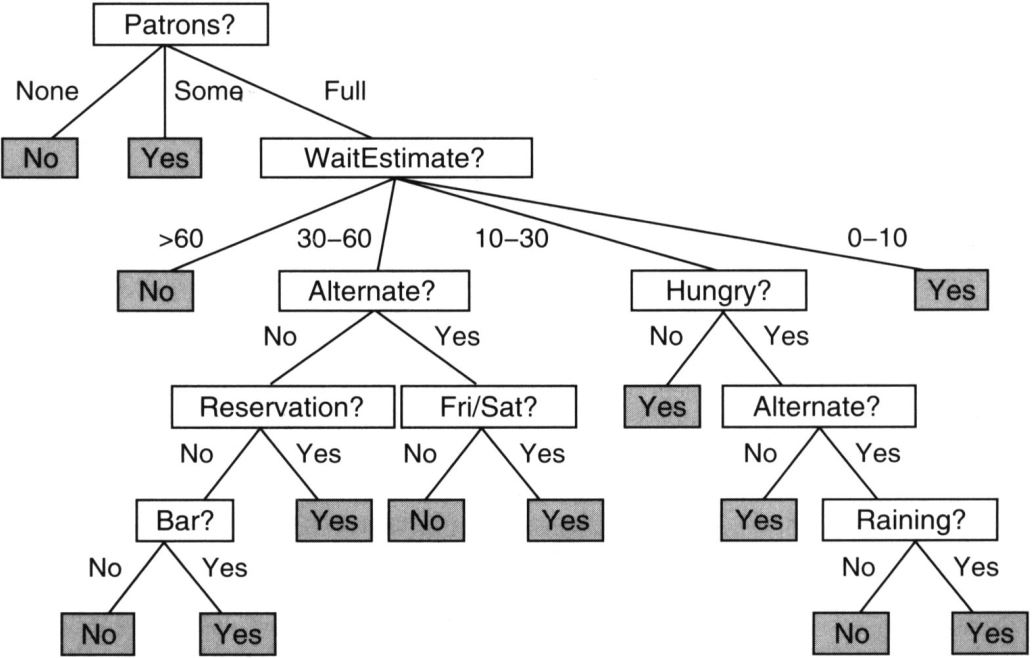
\includegraphics[width=0.5\linewidth]{figures/entscheidungsbaum.JPG}
	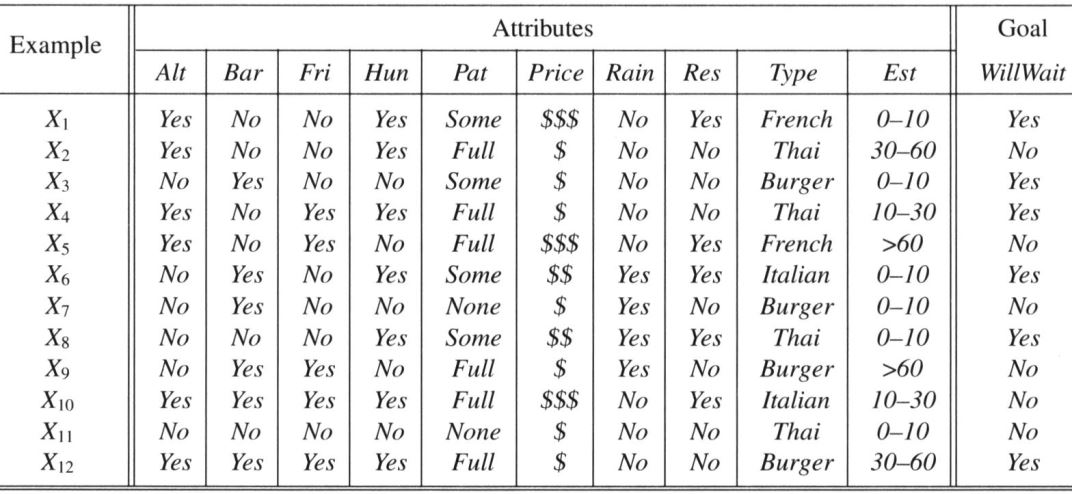
\includegraphics[width=0.5\linewidth]{figures/entscheidungsbaum-trainingsbeispiele.JPG}\\
	Für den Aufbau des Baums wähle Attribut aus der Trainingsmenge, das die meisten Zielzustände exakt vorhersagen kann/bedingt. Fahre rekursiv fort. Beispiel: für alle $Patrons = Some \Rightarrow WillWait = Yes$\\
	\textbf{Entropie in Entscheidungsbäumen} Für Entscheidungsbäume mit $p$ positiven und $n$ negativen Trainingsdatensätzen ergibt sich: $H(Ziel) = B(\frac{p}{p+n})$. Für ein Attribut $A$ mit $d$ verschiedenen Werten ergibt sich dann eine Entropie von: $Remainder(A) = \sum_{k=1}^{d} \frac{p_k + n_k}{p+n} B(\frac{p_k}{p_k + n_k})$. Die erwartete Entropiereduktion ist er Informationsgewinn des Attributs $A$ und beschreibt damit dessen Wichtigkeit (Entscheidungskriterium für bestes Attribut): $Gain(A) = B(\frac{p}{p+n}) - Remainder(A)$\\
	\textbf{Probleme} Unvollständige Daten $\rightarrow$ Werte schätzen, Attribute mit vielen Werten $\rightarrow$ Pruning\\
	
	% TODO continue with chapter 18, slide 32
	
\end{document}
